% ============================================================================
% The single-photon microwave loss of a moire superconducting element
% (P4, author-voice preprint for Zenodo / alphaXiv)
%
% Narrative (introduction, section openings, readings, conclusion): the
% author's own account, translated.  Equations, tables and numbers: taken
% from p4.tex with the corrections of the reference, claim and arithmetic
% checks applied (see yukleme_bilgisi.md).  Every computed number is
% recomputed by p4_yeniden_uretim.py except the readout-chain figures
% (from m30_loss.json); figures by fig_uret.py.  RevTeX 4.2.
% ============================================================================
\documentclass[aps,prb,reprint,superscriptaddress,longbibliography]{revtex4-2}

\usepackage{graphicx}
\usepackage{amsmath,amssymb}
\usepackage{silence}
% known, harmless RevTeX 4.2 + hyperref interaction
\WarningFilter{nameref}{The definition of \label has changed}
\usepackage[colorlinks=true,linkcolor=blue,citecolor=blue,urlcolor=blue]{hyperref}

\graphicspath{{figs/}}

% Zenodo (reserved) DOI
\newcommand{\zenododoi}{10.5281/zenodo.24204124}

\begin{document}

\title{The single-photon microwave loss of a moir\'e superconducting
element: why the published geometry cannot measure it, and a two-device
experiment that can}

\author{F. Sami Bilgin}
\thanks{\protect\raggedright Code and data: \href{https://doi.org/\zenododoi}{doi:\zenododoi}.}
\altaffiliation[Present affiliation: ]{Kocaeli University, Kocaeli, T\"urkiye}
\affiliation{Independent Researcher}

\date{\today}

\begin{abstract}
Moir\'e superconductors have entered superconducting circuits as
inductors, and everyone measures the wrong thing: how much inductance,
not how much energy is lost, and never at the single-photon level where
circuits operate. The published resonator measurements of
two-dimensional superconductors used as inductors were made in a
geometry that cannot measure the sample's own loss. This is not an error
of execution but a consequence of the geometry: the approximation that
extracts the kinetic inductance cleanly is the same approximation that
blinds the loss measurement, because the sample's dissipation enters
$1/Q_i$ multiplied by its participation $p$. On published numbers, and
on the reading that the fitted $Q_i$ and the 1\% shift belong to the
same superconducting device, everything that can be said about the
quality factor of a magic-angle element is $Q \geq 21$. The obstruction is removed by a mask line:
shortening the line until the sample is the resonator drives $p$ from
$0.02$ to $0.99998$. But then the contacts become the experiment,
$Q_{\rm contact} = Z/R_c$, and the length-ladder regression meant to
separate contact from intrinsic loss is degenerate once the gate
capacitance a moir\'e device cannot do without is budgeted; I publish
this here about my own design. What replaces it is a differential
measurement: one chip, one gate, one cooldown, two lumped resonators
matched in layout, one moir\'e and one base metal, and their difference. I give
the element, four controls, pre-registered decision rules, four outcome
bands, and the asymmetry that limits how far the number generalizes. I
have not performed the measurement; Sec.~\ref{sec:nomeas} says why.
\end{abstract}

\maketitle

% ============================================================================
\section{Introduction: everyone measures the wrong thing}
% ============================================================================

In the last few years moir\'e superconductors, magic-angle twisted
bilayer graphene (MATBG) first among them, have entered superconducting
circuits as inductive elements. Three groups measured them. Tanaka
\emph{et al.} terminated an Al $\lambda/4$ waveguide with a MATBG strip
and extracted the superfluid stiffness~\cite{Tanaka2025}. Banerjee
\emph{et al.} measured twisted trilayer graphene by rf reflectometry at
350\,MHz~\cite{Banerjee2025}. Jha \emph{et al.} measured a sheet kinetic
inductance tunable from 10 to 150\,nH per square with a single
gate~\cite{Jha2025}.

All three measure the reactive response: how much inductance. None of
them measures the dissipative response: how much energy is lost; and
none at all at the single-photon level where circuits actually operate.

That is the number that decides. For a fluxonium whose inductor is a
moir\'e strip, $T_1 = 100\,\mu$s requires $Q_{\rm ind} \geq 3.218 \times
10^{6}$; if $T_1 = 1\,\mu$s is enough, $3.218 \times 10^{4}$ suffices
(assumptions in Sec.~\ref{sec:meaning}). Two orders of magnitude apart,
and for no moir\'e element does the literature distinguish between the
two.

The first argument below (Sec.~\ref{sec:geometry}) does not depend on
any device of mine: only published numbers and a closed-form expression.
It is the stronger half of the paper. The rest is a measurement design,
including the place where it refutes its own earlier version.

% ============================================================================
\section{The published geometry cannot measure it, and structurally so}
\label{sec:geometry}
% ============================================================================

\subsection{The exact expression}

A lossless line of impedance $Z_0$ is terminated at one end by an
inductance $L$, the sample, and open at the other. With the current
$I(z) = A\cos(\beta z + \varphi)$ measured from the terminated end, the
boundary condition $V(0)/I(0) = j\omega L$ gives
\begin{equation}
\tan\varphi = \omega L/Z_0 ,
\label{eq:phi}
\end{equation}
and the open end requires $\beta l + \varphi = \pi/2$. The participation
ratio, the fraction of the mode's inductive energy stored in the sample,
follows from integrating the magnetic energy along the line:
\begin{equation}
p(\varphi) = \frac{\sin 2\varphi}{\sin 2\varphi/2 + (\pi/2 - \varphi)} .
\label{eq:p}
\end{equation}
It has two limits. For $\omega L \ll Z_0$ it reduces to
$p = 2|\delta\omega/\omega|$, the factor that weights $\tan\delta$ in
Eq.~(9) of Kreidel \emph{et al.}~\cite{Kreidel2024} (they call
$|\delta\omega/\omega|$ itself the participation ratio, normalized to
the total stored energy). To first order this holds for any layout: a
sample that shifts the resonance by $\delta\omega/\omega$ carries
$p \approx 2|\delta\omega/\omega|$ of the inductive energy. For
$\omega L \gg Z_0$, and only then, $p$ approaches 1.

\begin{table}[!tbp]
\caption{\label{tab:p}Participation of a terminating inductance, exact
[Eq.~(\ref{eq:p})] and perturbative, with the resonant line length as a
fraction of $\lambda/4$. Computed.}
\begin{ruledtabular}
\begin{tabular}{cccc}
$\omega L/Z_0$ & $p$ (exact) & $2|\delta\omega/\omega|$ & length$/(\lambda/4)$ \\
\hline
0.01 & 0.0127 & 0.0127 & 0.994 \\
0.3  & 0.354  & 0.371  & 0.815 \\
1.0  & 0.778  & 1.000  & 0.500 \\
10   & 0.9967 & 1.873  & 0.064 \\
\end{tabular}
\end{ruledtabular}
\end{table}

The exact $p$ crosses one half at $\omega L/Z_0 = 0.46$, reaches 0.99 at
5.7 and 0.997 only at 10.5 (Table~\ref{tab:p}, Fig.~\ref{fig:p}). The
perturbative form stays within 5\% of it only up to $\omega L/Z_0
\approx 0.3$, where $p \leq 0.354$; above $\omega L/Z_0 = 1$ it exceeds
unity and means nothing.

\subsection{The trap}

The geometry that makes $p$ small is the geometry in which the sample
perturbs a known resonator by a small, cleanly interpretable amount.
That is exactly what one wants for extracting $L_k$. And it is exactly
what kills the loss measurement, because the sample's dissipation enters
$1/Q_i$ multiplied by $p$.

The approximation is not a detail of the method; it is the method.

\begin{figure}[!tbp]
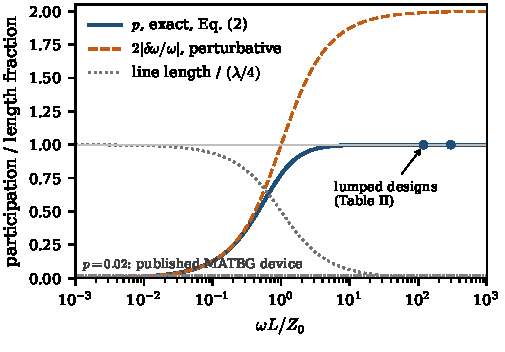
\includegraphics[width=\columnwidth]{fig1_participation.pdf}
\caption{\label{fig:p}Participation of a terminating inductance versus
$\omega L/Z_0$: exact, Eq.~(\ref{eq:p}) (solid); perturbative
$2|\delta\omega/\omega|$ (dashed); resonant line length in units of
$\lambda/4$ (dotted). The dash-dotted line marks $p = 0.02$, read from
the measured shift of the published MATBG device~\cite{Tanaka2025}; the
dots are two of the lumped designs of Table~\ref{tab:design}.}
\end{figure}

There is no error of execution here. The geometry structurally cannot do
both things at once, and there is no intermediate regime either;
Table~\ref{tab:p} shows it.

\subsection{The published device, scored}
\label{sec:tanaka}

The MATBG resonator of Tanaka \emph{et al.} has $Q_i = 1044.7 \pm 28.5$
and $Q_c = 4161$ at $f_r = 4.2008154$\,GHz; an Al control on the same chip
has $Q_i = 74\,833$~\cite{Tanaka2025}. The resonance shifts by about 1\%
between the insulating and superconducting states, so $p = 0.02$. In
their circuit model the strip does not terminate the line alone: it sits
in parallel with a proximitized-graphene inductance $L_{\rm prx} =
1.32$\,nH at the contacts~\cite{Tanaka2025}, so $p$ is set by the
current division between the two, and is read from the measured shift
rather than from $\omega L/Z_0$ of the strip.

From these numbers, $Q_{\rm MATBG} \geq 20.9$ by direct dilution and
$\geq 21.2$ by the excess-loss argument (subtracting the control's
loss), i.e.\ $\tan\delta \leq 4.79 \times 10^{-2}$. One caveat belongs
to the source: the fitted resonance at 4.2008\,GHz lies outside the
3.80--3.86\,GHz band of the device whose $\sim\!1\%$ shift fixes $p$
(nominal $f_0 = 3.8$\,GHz), and close to the high-resistance baseline of
their second device; the source does not state which device or gate
point the fit belongs to, so the bound assumes that $Q_i$ and $p$ refer
to the same device in the superconducting state. No choice of $p$
rescues the number: even at $p = 1$ the bound could not exceed $Q_i$
itself, about 1045, thirty times below the weakest circuit threshold.

This is an important nuance: it is not a null result. It is the only quantitative statement
about moir\'e microwave loss that the literature supports. Tanaka
\emph{et al.}'s paper should therefore be cited with its number, not
with ``no data''. Their own framing is honest: the platform is
``capable of discerning changes in the superfluid stiffness at the 1\%
level''~\cite{Tanaka2025}. It was built to measure $L_k$, and it
measures $L_k$. It is not to blame for not doing what it did not set out
to do.

Two notes on it. The photon number at which $Q_i$ was taken is not
stated: power is swept against the resonance frequency and dc bias
current against $Q_i$ (their Fig.~5d and Supplementary Fig.~17 in the
arXiv version), but
$Q_i$ versus microwave power appears nowhere. And their simulation fixes
the MATBG--back-gate capacitance at 3\,fF, a value estimated from the
dimensions and dielectric constant of the bottom hBN, not
measured~\cite{Tanaka2025}. That number will later kill a design.

\subsection{A measurement of this kind has already said it about itself}

Kreidel \emph{et al.}, whose author list overlaps that of the trilayer
measurement~\cite{Banerjee2025}, probed Al and NbSe$_2$ strips with a Nb
$\lambda/4$ resonator of bare $Q_0 \approx 10^{5}$~\cite{Kreidel2024}.
In their own paper they write:
\begin{quote}
``Since the participation ratio of the sample is merely a few ppt, the
probe resonator quality factor $Q_0$ is too low for us to discern the
true $Q$ factor of the sample component.''~\cite{Kreidel2024}
\end{quote}
(The statement is made for their NbSe$_2$ data at temperatures
approaching the $T_c$ of Nb.) This is very valuable. This paper attacks
no one: one of the two resonator measurements has already admitted the
problem in writing. I only show that it is not an accident but a
necessity of the geometry.

The measurement has been done at the single-photon level on a
van der Waals superconductor that is not moir\'e. Zaman \emph{et al.}
measured twelve hBN-encapsulated NbSe$_2$ strips terminating Al
$\lambda/4$ resonators at 10\,mK, beside an Al spectator at $Q_i = 5.985
\times 10^{6}$~\cite{Zaman2026}. Their device D2 ($L_k = 0.643$\,nH,
$Q_i = 6.0 \times 10^{4}$) has $p = 0.3885$ by Eq.~(\ref{eq:p}), so
$\tan\delta \leq 1/(pQ_i) = 4.3 \times 10^{-5}$ without subtracting any
background, the strongest bound among their twelve devices (computed
here). Their $Q_i$ scatters up to about sevenfold at comparable $L_k$, which
they attribute to ``imperfect electrical contacts between the Al and the
NbSe$_2$, as well as dielectric loss introduced by residual polymer
contamination from the dry transfer process''~\cite{Zaman2026}. A
design that cannot separate extrinsic from intrinsic loss in situ will
report the extrinsic number as a material property.

% ============================================================================
\section{The fix is a mask line}
\label{sec:fix}
% ============================================================================

As $\omega L/Z_0$ grows, the resonant length collapses. At 5.5\,GHz a
moir\'e strip of 430.71\,nH gives $\omega L/Z_0 = 297.7$ against
50\,$\Omega$, and the resonant stub is 11.57\,$\mu$m long, against a
quarter wave of 5.4\,mm at the same frequency and effective permittivity
(7.1\,mm at the 4.2\,GHz of Ref.~\cite{Tanaka2025}).

Nothing changes in fabrication. The stack, the encapsulation, the edge
contacts, the base metal and the gate are all the published
ones~\cite{Tanaka2025,Zaman2026}. Only the length of one line on the
mask changes.

The device stops being a ``perturbed transmission-line resonator'' and
becomes a lumped $LC$ resonator whose entire inductance is the sample.
Table~\ref{tab:design} lists the elements; for the one chosen in
Sec.~\ref{sec:diff}, $p = 0.99998$.

\begin{table}[!tbp]
\caption{\label{tab:design}Lumped moir\'e resonators at an assumed sheet
inductance $L_\Box = 29.3$\,nH/$\Box$ (inside the window of
Ref.~\cite{Jha2025}); $N$ is the number of squares, $C = 1/(\omega^2
L)$ the total capacitance the element allows, $Z = \sqrt{L/C}$. All
have $p \geq 0.99989$. $C/A$ is $C$ per moir\'e area, and $t_{\min}$ the
bottom-hBN thickness above which a parallel-plate gate under the whole
strip stays below $C$ ($\varepsilon_\perp = 3.76$~\cite{Laturia2018}).
Computed, not measured.}
\begin{ruledtabular}
\begin{tabular}{rrrrrrrr}
$N$ & $w$ & $L$ & $f_r$ & $C$ & $Z$ & $C/A$ & $t_{\min}$ \\
 & (nm) & (nH) & (GHz) & (fF) & (k$\Omega$) & (fF/$\mu$m$^2$) & (nm) \\
\hline
2    & 903.7 & 58.6   & 7.50 & 7.685 & 2.76  & 4.70  & 7.1 \\
5    & 532.1 & 146.5  & 6.50 & 4.092 & 5.98  & 2.89  & 11.5 \\
14.7 & 400.0 & 430.71 & 5.50 & 1.944 & 14.88 & 0.83  & 40 \\
40   & 400.0 & 1172   & 4.50 & 1.067 & 33.14 & 0.17  & 200 \\
100  & 400.0 & 2930   & 3.80 & 0.599 & 69.96 & 0.037 & 890 \\
\end{tabular}
\end{ruledtabular}
\end{table}

The strip width follows from phase headroom: with $\xi \leq 200$\,nm
and a sheet critical current of 200\,nA/$\mu$m~\cite{Jha2025}, the
widths of Table~\ref{tab:design} keep the zero-point phase at least a
factor of 3 below the phase the strip can hold, and the zero-point current at one
photon at most 3.6\% of the sheet depairing current. Every element is a
linear resonator at one photon.

% ============================================================================
\section{But then the contacts become the experiment}
\label{sec:contacts}
% ============================================================================

Raising $p$ from 0.02 to 1 buys a factor 50, and no more. The moment the
sample carries all the inductive energy, the galvanic contacts are in
series with the whole resonant current:
\begin{equation}
Q_{\rm contact} = \omega L/R_c = Z/R_c ,
\label{eq:qc}
\end{equation}
with $R_c = 2\rho_c/W_{\rm pad}$ for two contacts of width $W_{\rm pad}
= 10\,\mu$m (Table~\ref{tab:contacts}).

\begin{table}[!tbp]
\caption{\label{tab:contacts}Contact-limited quality factor across the
elements of Table~\ref{tab:design}. Computed.}
\begin{ruledtabular}
\begin{tabular}{rrlp{0.42\columnwidth}}
$\rho_c$ ($\Omega\,\mu$m) & $R_c$ ($\Omega$) & $Q_{\rm contact}$ & \raggedright basis \tabularnewline
\hline
100 & 20 & 138--3498 & \raggedright edge contact to a 2D crystal at its demonstrated value (normal-state graphene)~\cite{Wang2013} \tabularnewline
1\,000 & 200 & 13.8--350 & \raggedright tenfold worse, for the low carrier density of the flat band \tabularnewline
16\,000 & 3\,200 & 0.9--21.9 & \raggedright the published moir\'e rf contact value, 3.2\,k$\Omega$~\cite{Banerjee2025}, applied unchanged at the 10\,$\mu$m pad (no benefit from the pad) \tabularnewline
\end{tabular}
\end{ruledtabular}
\end{table}

The third row is the risk if the published 3.2\,k$\Omega$ does not
scale with contact width. Banerjee \emph{et al.} measured the rf
resistance of a twisted-trilayer element at 350\,MHz and found that in
the superconducting state ($R_{4t} = 0$) $R_{\rm rf} \approx R_{2t}
\approx R_c \approx 3.2$\,k$\Omega$, arising purely from the contact
resistance~\cite{Banerjee2025}. I infer that the element's own
dissipation sits below that floor and cannot be extracted. At that
resistance every element in the design set is pinned below $Q \approx
22$.

If it does scale, the cheapest cure is a layout change: the contact need not be as narrow
as the strip: flaring the moir\'e into a 10\,$\mu$m pad at each end cuts
$R_c$ by up to 25 times (18.8 times for the element chosen below), at
the cost of a fraction of a square.

If the 3.2\,k$\Omega$ is instead a fixed, lumped interface resistance, no
pad helps and the galvanic design is dead from the start. This can be
tested with a dc four-probe measurement before the rf chip is cooled, and
it is pre-registered as rule K0 in Table~\ref{tab:rules}.

Figure~\ref{fig:q} puts these ceilings on one scale with the bounds of
Sec.~\ref{sec:geometry} and the outcome bands of
Sec.~\ref{sec:meaning}.

\begin{figure}[!tbp]
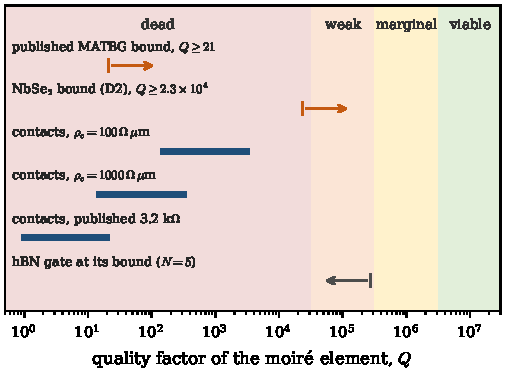
\includegraphics[width=\columnwidth]{fig2_q_scale.pdf}
\caption{\label{fig:q}Quality-factor scale of a moir\'e element. Shaded:
the four outcome bands of Table~\ref{tab:bands}. Arrows to the right:
lower bounds computed from published data (MATBG~\cite{Tanaka2025};
NbSe$_2$ device D2~\cite{Zaman2026}). Bars: contact ceilings of
Table~\ref{tab:contacts}. Arrow to the left: the cap set by the hBN gate
dielectric if its loss tangent sits at its published upper
bound~\cite{Wang2022} (Sec.~\ref{sec:refute}).}
\end{figure}

% ============================================================================
\section{Where the paper refutes its own design}
\label{sec:refute}
% ============================================================================

The natural way to separate the two losses is a length ladder. At fixed
contact geometry the inductance and the intrinsic series resistance
scale with $N$, while $R_c$ does not:
\begin{equation}
1/Q_i(N) = \tan\delta_{\rm intrinsic} + \frac{R_c}{\omega L_\Box N} .
\label{eq:ladder}
\end{equation}
In the regression, the intercept is the intrinsic loss and the slope is
the contact resistance. The arithmetic works: with 1\% uncertainty per
point over the five elements of Table~\ref{tab:design}, the $3\sigma$
floor on the intrinsic loss tangent is $1.09 \times 10^{-5}$ at $\rho_c
= 100\,\Omega\,\mu$m (for vanishing intrinsic loss).

But it is correct arithmetic on a device that cannot be realised.

\subsection{The obstacle is the gate}

A floating moir\'e island can be given a displacement field but not a
filling factor: a top and a bottom gate induce equal and opposite
surface charge, and the net density does not change. MATBG without
control of $\nu$ is useless, so the gate capacitance is mandatory. For a
real device of this class, Tanaka \emph{et al.}'s simulation uses
3\,fF~\cite{Tanaka2025}, an estimate rather than a measurement
(Sec.~\ref{sec:tanaka}).

Three of the five elements, $N = 14.7$, 40 and 100, specify a
\emph{total} resonator capacitance of 1.944, 1.067 and 0.599\,fF, below
that one mandatory contribution. And they are exactly the three that
carry the $1/N$ lever. Since the gate capacitance scales with area, the
fair comparison is per area (Table~\ref{tab:design}): the $N = 40$ and
$N = 100$ rungs survive only above 200 and 890\,nm of bottom hBN, the
$N = 14.7$ rung above 40\,nm, while $N = 5$ needs only 11.5\,nm.

Worse, the problem is not only realisability but structure. Once the
gate dominates $C$, at fixed strip width $C_{\rm gate} \propto N$ and
$L = L_\Box N$, so $Z = \sqrt{L/C}$ becomes independent of $N$, and the
contact term $R_c/Z$ freezes with it. The design matrix of
Eq.~(\ref{eq:ladder}) is degenerate. The claimed 50-fold lever (in $N$;
25-fold in the regressor itself, since the frequency changes along the
ladder) exists only under a capacitance that cannot be realised.

\subsection{The second consequence, and the heavier one}

If $C \approx C_{\rm gate}$, the hBN gate dielectric carries nearly all
of the mode's electric energy. The loss tangent of hBN is bounded only
from above, $\tan\delta_{\rm hBN} \leq 5 \times 10^{-6}$ at one photon
and 10\,mK~\cite{Wang2022}. If it sits at that bound, the gate alone
(electric participation $3/4.092 = 0.73$ for the $N = 5$ element, with
the 3\,fF estimate) caps $Q_i$ near $2.7 \times 10^{5}$, below the
$3.2 \times 10^{5}$ threshold of rule K4 at which the experiment could
declare the route unblocked. The published bound cannot exclude this,
so the experiment is not guaranteed to be able to unblock the route.

The ceiling of any measurement in this class may be set not by the
moir\'e but by the gate dielectric. I state it before a referee finds it.

\subsection{What survives}

The participation critique, the stub-shortening fix, and the two
elements whose total capacitance exceeds the 3\,fF estimate and whose
per-area budget survives any bottom hBN thicker than 7.1 and 11.5\,nm:
$N = 2$ (7.685\,fF) and $N = 5$ (4.092\,fF). What does not survive is the
regression itself.

% ============================================================================
\section{Differential, not regression}
\label{sec:diff}
% ============================================================================

\begin{quote}
On one chip, over one back gate of a single measured hBN thickness, two
lumped resonators matched in layout, with the same 10\,$\mu$m flared
contact geometry and the same coupling capacitors. In one the
inductor is a magic-angle moir\'e strip; in the other a base-metal (Nb)
bar. $Q_i$ of both is extracted for photon numbers from 0.1 to $10^{6}$,
at 20\,mK, in the same cooldown, on the same feedline.
\end{quote}

The twin isolates, in place and without any fit model, everything a
regression would eliminate by assumption: the loss of the hBN gate
dielectric at its true participation, coupling-capacitor loss, and
package loss. Contact loss enters as $R_c/Z$ and does not cancel,
because the twin has a different $Z$ and no moir\'e--metal interface;
it is subtracted using $R_c$ from the companion Hall bar, and the
differential can reach the K3 (K4) threshold only if $\rho_c \lesssim 1$
($0.1$)\,$\Omega\,\mu$m at the 10\,$\mu$m pads, i.e.\ effectively
non-dissipative contacts. With that term removed from the moir\'e arm,
the moir\'e loss is the difference in $1/Q_i$,
\begin{equation}
p\,\tan\delta_{\rm moir\acute{e}} = 1/Q_i({\rm moir\acute{e}}) -
1/Q_i({\rm twin}),
\label{eq:diff}
\end{equation}
taken at matched photon number and temperature, with $p = 0.99998$, so
the participation correction is a rounding error rather than a model. No
regressor, no assumption about how $C$ or $Z$ scales, no extrapolation.

The chosen element is $N = 5$: a $532.1\,{\rm nm} \times 2.66\,\mu$m
strip of 146.5\,nH at 6.5\,GHz, $C = 4.092$\,fF, $Z = 5.98$\,k$\Omega$,
$p = 0.99998$, $hf/k_B = 312$\,mK, on 1.416\,$\mu$m$^2$ of moir\'e. The
reason for the choice: its 4.092\,fF exceeds the 3\,fF estimated for a
device of this class, and per area it survives any bottom hBN thicker
than 11.5\,nm.

\subsection{Four controls}

None of them needs an extra process module or line.
\begin{enumerate}
\item \emph{The base-metal twin}, the reference arm of the differential.
Its decision role comes before everything else: if the twin's own $Q_i$
is below $3.2 \times 10^{5}$, the extrinsic floor is already above the
threshold.
\item \emph{A bare base-metal reference resonator}, expected near
$10^{6}$; Zaman \emph{et al.} measured $5.985 \times 10^{6}$ for the
equivalent structure~\cite{Zaman2026}. It separates a chip problem from
a sample problem.
\item \emph{The same moir\'e strip gated out of the dome}, to the
correlated insulator at $\nu = +2$ and to charge neutrality. This is the
one control the moir\'e platform can perform and no thin film can: it
asks directly whether the loss belongs to the superconducting state.
\item \emph{A companion Hall bar on the same flake}, giving $T_c$, $\nu$,
sheet resistance, contact resistance, and the twist angle from the
Landau fan, in the same cooldown. This is what makes the resonator data
interpretable, and $R_c$ is screened on it in a dc cooldown before the
rf chip is cooled.
\end{enumerate}

\subsection{Extraction, sweeps and cost}

$Q_i$ comes from the circle fit of Probst \emph{et
al.}~\cite{Probst2015} with point placement per Baity \emph{et
al.}~\cite{Baity2024}; the photon number is $\bar n = 2\kappa P_{\rm
rf}/[\hbar\omega_r(\kappa+\gamma)^2]$, as in Zaman \emph{et al.}'s
Supplementary Eq.~(3)~\cite{Zaman2026} after Norris \emph{et
al.}~\cite{Norris2024}. Because fit precision degrades as
$1 + Q_i/Q_c$ and $Q_i$ is the unknown, each element is drawn twice,
with $Q_c = 10^{4}$ and $10^{6}$.

Fifteen power points span $\bar n = 0.1$--$10^{6}$; twelve temperatures
span 20\,mK--1.2\,K. $Q_i$ rising with power roughly as $\sqrt{1 + \bar
n/n_c}$ means two-level systems; a flat $Q_i(\bar n)$ means resistive
loss: contacts, normal regions of twist disorder, or
quasiparticles~\cite{McRae2020}. The design band puts $hf/k_B$ between
182 and 360\,mK, so a two-level-system peak like the one Kreidel
\emph{et al.} saw near 0.2\,K on their Al-strip
resonator~\cite{Kreidel2024} falls inside the sweep; a fall tracking
$\exp(-\Delta/k_BT)$ toward $T_c \approx 1$\,K~\cite{Tanaka2025} is the
quasiparticle signature. Flat in both means a fabrication problem, and
it must be reported as one, not as a material number.

The chain is one rf line in, one out, four dc lines, no fast lines, and
80\,dB of attenuation, leaving a computed residual thermal occupancy of
$5.17 \times 10^{-3}$ at the sample. The computed acquisition budget,
4.19\,h for the ten-resonator campaign of the companion data (of which
this chip is a subset) at a system noise of three quanta, is dominated
by temperature settling (4.0\,h) rather than signal-to-noise; with a
HEMT alone (about twelve quanta) only the signal-limited part grows,
roughly fourfold, so a parametric amplifier is optional. The measurement is an afternoon; the
schedule is fabrication and cooldowns.

Fabrication takes six process modules, all published: a 240\,nm
sputtered Nb base layer on float-zone Si~\cite{Kreidel2024} (or 250\,nm
MBE Al on high-resistivity Si~\cite{Zaman2026}); a Ti/Al back gate by
e-beam lithography in the resonator cutout~\cite{Tanaka2025}; the
magic-angle stack by dry polymer transfer, chloroform polymer removal
and contact-mode AFM cleaning~\cite{Tanaka2025}; strip and Hall-bar
patterning; edge contacts by RIE, in-situ ion milling and Al at a
30$^\circ$ tilt with substrate rotation~\cite{Zaman2026} (or Ti/Al by
thermal evaporation~\cite{Tanaka2025}); and the capacitors in the base
metal. The twin needs no seventh module: its inductor is drawn in the
base layer.

\begin{table}[!tbp]
\caption{\label{tab:rules}Decision rules fixed before the chip is cooled,
including the one under which the experiment declares itself void.}
\begin{ruledtabular}
\begin{tabular}{lp{0.27\columnwidth}p{0.55\columnwidth}}
id & \raggedright test & \raggedright outcome \tabularnewline
\hline
K0 & \raggedright dc four-probe $R_c$, before the rf cooldown & \raggedright $\rho_c > 1000\,\Omega\,\mu$m ($R_c > 200\,\Omega$): do not cool the rf chip; refabricate with wider pads. If $R_c$ does not fall with width, the interface is lumped and the galvanic design is dead \tabularnewline
K1 & \raggedright gated-out control & \raggedright $Q_i$ unchanged: the resonator does not see the moir\'e; measurement void \tabularnewline
K1$'$ & \raggedright the twin's $Q_i$ & \raggedright $< 3.2 \times 10^{5}$: extrinsic floor above threshold; report the floor \tabularnewline
K2 & \raggedright difference vs.\ its $3\sigma$ & \raggedright consistent with zero: only the extrinsic channel is bounded; refabricate \tabularnewline
K3 & \raggedright $\tan\delta$ at $\bar n = 1$ & \raggedright $> 3.1 \times 10^{-5}$ ($Q < 3.2 \times 10^{4}$) on two flakes, loss tracking the superconducting state: route dead \tabularnewline
K4 & \raggedright $\tan\delta$ at $\bar n = 1$ & \raggedright $\leq 3.1 \times 10^{-6}$ ($Q \geq 3.2 \times 10^{5}$): route unblocked \tabularnewline
K5 & \raggedright $Q_i(\bar n)$, $Q_i(T)$ & \raggedright flat in both below $T_c$: contacts or twist-disorder normal regions; the cure is fabrication \tabularnewline
\end{tabular}
\end{ruledtabular}
\end{table}

The decade between K3 and K4 is deliberately left without a verdict: a
loss tangent there means $T_1 = 1$--$10\,\mu$s, publishable physics, but
not a basis for either continuing or cancelling a circuit programme.

% ============================================================================
\section{What the number would mean}
\label{sec:meaning}
% ============================================================================

For an inductively shunted qubit,
\[
\Gamma_1 = (2E_L/\hbar)(1/Q_{\rm ind})|\langle 0|\hat\varphi|1\rangle|^2 .
\]
The thresholds in the
introduction use $E_L/h = 0.38$\,GHz (an inductance near 430\,nH) and
$|\langle 0|\hat\varphi|1\rangle| = 2.5959$ for a fluxonium at half flux
quantum, with $T \to 0$; at finite temperature the requirement rises by
$\coth(hf_{01}/2k_BT)$, and I assume $Q_{\rm ind}$ does not depend on
frequency between the resonator band and the qubit transition, and I
assign the whole $T_1$ budget to inductive loss (conventions for the
prefactor differ by a factor of 2 in the literature). Because a
superinductor has $p \approx 1$, the $Q_i$ this experiment extracts
\emph{is} $Q_{\rm ind}$. Table~\ref{tab:bands} gives four bands, with
the priors written openly; the thresholds are rounded from $3.218$.

\begin{table}[!tbp]
\caption{\label{tab:bands}Four outcome bands; each band runs from its
lower edge to the edge of the band above.}
\begin{ruledtabular}
\begin{tabular}{llll}
band & $Q_i$ & $T_1$ ($\mu$s) & reading \\
\hline
viable   & $\geq 3.2 \times 10^{6}$ & $\geq 100$ & speculative \\
marginal & $\geq 3.2 \times 10^{5}$ & 10--100 & not competitive \\
weak     & $\geq 3.2 \times 10^{4}$ & 1--10 & most likely \\
dead     & $< 3.2 \times 10^{4}$ & $<1$ & fits all data \\
\end{tabular}
\end{ruledtabular}
\end{table}

\emph{Viable} would put the material with the best lumped
high-kinetic-inductance elements measured, granular aluminium at $Q_i =
3.66 \times 10^{6}$ (all-grAl) and $4.72 \times 10^{6}$ (hybrid
grAl/Ta) at one photon~\cite{Gupta2025}. I mark it as speculation: no
van der Waals Josephson or inductive element has been measured better
than $\tan\delta = 1.7 \times 10^{-5}$~\cite{Balgley2025}, 55 times
worse than this band requires (hBN as a dielectric is bounded at $5
\times 10^{-6}$~\cite{Wang2022}). \emph{Marginal} is worth building but
not competitive with a planar (2D) transmon at $T_1 \approx 1$\,ms~\cite{Bland2025}.
\emph{Weak} is where the literature sits, at its lower edge:
all-van-der-Waals transmons at mean $T_1 = 1.11$ and
$1.67\,\mu$s~\cite{Balgley2025}, with a graphene superconducting qubit
just below it at $T_1 = 716 \pm 17$\,ns at a single gate
point~\cite{Aparicio2025}. It is the most likely outcome, and I say so
here. \emph{Dead} is consistent with everything published so
far, including the $Q \geq 21$ of Sec.~\ref{sec:tanaka}.

\subsection{The asymmetry that limits the generalization}

What I call the dilution escape~\cite{Balgley2025} is
$T_1 = 1/(2\pi f p \tan\delta)$. At $\tan\delta = 3.1 \times 10^{-5}$, an
element with $p = 1\%$ in a 6\,GHz qubit gives $T_1 = 85.57\,\mu$s
instead of $0.86\,\mu$s. (The fluxonium mapping above gives $1\,\mu$s
for the same loss tangent because its prefactor corresponds to
5.1\,GHz.) Balgley \emph{et al.} make this argument for their own
junction, and they are right.

But it works for a junction or a capacitor, not for a superinductor,
because the whole function of a superinductor is to carry nearly all of
the inductive energy. $p \approx 1$ cannot be relaxed. So this number
closes \emph{hard} every superinductor, $\cos 2\varphi$ element,
resonator, kinetic-inductance detector and parametric amplifier whose
inductor is moir\'e; \emph{softly} the dispersive readout of a
topological device, whose resonator can be niobium; and \emph{not at
all} topological physics itself. I do not claim that it does.

% ============================================================================
\section{Why this paper contains no measurement}
\label{sec:nomeas}
% ============================================================================

The single-photon loss tangent of a moir\'e element has not been
measured. This paper does not report it, does not estimate it, and does
not bound it beyond $Q \geq 21$. The argument of
Sec.~\ref{sec:geometry} depends on no device of mine, and holds whether
or not a chip is ever cooled. The design of Secs.~\ref{sec:fix}--\ref{sec:diff}
is a specification, not a result. If the reader's threshold for
publication is this number, this paper is below it.

% ============================================================================
\section{Limitations}
% ============================================================================

\begin{enumerate}
\item \emph{No data.} Every quantity called computed or designed is
arithmetic on a closed form or on published inputs.
\item \emph{The gate dielectric may set the ceiling}
(Sec.~\ref{sec:refute}); the hBN loss tangent is known only as an upper
bound.
\item \emph{The capacitance argument rests on an estimate.} The 3\,fF is
a simulation input of one device~\cite{Tanaka2025}. The degeneracy
($Z$ independent of $N$ once the gate dominates) is geometric and does
not depend on it; which rungs survive depends on the hBN thickness
(Table~\ref{tab:design}), and $\varepsilon_\perp = 3.76$ is a
first-principles value~\cite{Laturia2018}.
\item \emph{The twin is not inductance-matched.} A Nb bar cannot be
drawn with 146.5\,nH, so the twin resonates at another frequency and
frequency-dependent channels, two-level systems above all, are
subtracted only approximately. With the same 4.092\,fF shunt a twin
would need at least 110\,nH to resonate below 7.5\,GHz, so its shunt
capacitor must differ, and with it the participation of the gate
dielectric.
\item \emph{The contacts must be nearly lossless.} For the chosen
element $Z = 5.98$\,k$\Omega$, so even the best demonstrated edge
contact (Table~\ref{tab:contacts}) caps $Q$ near 300; the thresholds of
Table~\ref{tab:bands} are reachable only with $\rho_c \lesssim
1\,\Omega\,\mu$m, two orders below the best value in
Table~\ref{tab:contacts}.
\item \emph{The contact conversion is assumption-laden.} The only
published moir\'e rf contact number is a total
3.2\,k$\Omega$~\cite{Banerjee2025}, whose contact width I do not have.
\item \emph{The material inputs are borrowed.} The sheet inductance
window, critical current and $\xi$ come from magic-angle twisted
trilayer graphene at 1.71$^\circ$~\cite{Jha2025}; Table~\ref{tab:design}
moves if the bilayer differs.
\item \emph{The schedule risk is the stack, not the measurement.}
Twist-angle disorder inside finished MATBG devices has been mapped
directly, with local spans approaching 0.1$^\circ$~\cite{Uri2020}.
\end{enumerate}

% ============================================================================
\section{Conclusion}
% ============================================================================

The published resonator measurements of two-dimensional superconductors
used as inductors were made in a geometry that cannot measure the
sample's own loss, and this is not an error of execution but a
consequence of the geometry: the approximation that extracts $L_k$
cleanly is the same one that blinds the loss. With published numbers,
and on the reading that the fitted $Q_i$ and the 1\% shift belong to
the same superconducting device, everything that can be said about the
quality factor of a magic-angle element is $Q \geq 21$. The obstruction is removed by a mask line, but
at that moment the contacts become the experiment; and the length-ladder
regression thought to solve this is degenerate once the gate capacitance
a moir\'e device cannot do without is budgeted. I publish this here,
about my own design. What replaces it is a differential measurement: one
chip, one gate, one cooldown, two lumped resonators matched in layout,
one moir\'e and one base metal, and their difference. I have not performed the
measurement; Sec.~\ref{sec:nomeas} says why.

\begin{acknowledgments}
The manuscript was written from the author's own account of the work;
Claude (Anthropic) was used for coding, literature search, and for
translating and editing the author's text into English. The study and its
computational workflows were conceived and directed by the author, who
chose the methods, targets, and computational stages, provided and
configured the computing environment, verified all results and
references, and bears sole responsibility for the content.
\end{acknowledgments}

\section*{Data availability}
{\raggedright
No new measurements were made. The computed numbers are in two files,
\texttt{m30\_loss.json} (participation, design, contacts, chain,
thresholds) and \texttt{m31\_route\_ranking.json} (the gate-capacitance
comparison). The participation, bound, design, contact, regression,
threshold and band numbers are recomputed independently, without reading
those files, by \texttt{p4\_yeniden\_uretim.py}; the figures are drawn by
\texttt{fig\_uret.py}. The two JSON files are regenerated exactly by the
project scripts \texttt{run\_m30\_loss.py} and
\texttt{run\_m31\_route\_ranking.py}, which are deterministic and need
only NumPy. All six files are in the Zenodo record,
\href{https://doi.org/\zenododoi}{doi:\zenododoi}. The independent
script checks every number used here except the readout-chain figures
(the attenuation, the residual thermal occupancy and the acquisition
budget), which are taken from \texttt{m30\_loss.json}. Several descriptive and
bibliographic fields in \texttt{m30\_loss.json} predate the checks behind
this version (among them an author list, a reading of the participation
curve, a quarter-wave length, the arXiv-version $Q_i$ of one NbSe$_2$
device, the amplifier attributions, the contact-width label, and the
fabrication-recipe attributions); an errata file in the record,
\texttt{ERRATA.txt}, lists them, and where they differ, this text and
the independent script are correct.\par}

% ============================================================================
\begin{thebibliography}{99}
\raggedright

\bibitem{Tanaka2025}
M.~Tanaka, J.~\^{I}-j.~Wang, T.~H.~Dinh, D.~Rodan-Legrain, S.~Zaman,
M.~Hays, A.~Almanakly, B.~Kannan, D.~K.~Kim, B.~M.~Niedzielski,
K.~Serniak, M.~E.~Schwartz, K.~Watanabe, T.~Taniguchi, T.~P.~Orlando,
S.~Gustavsson, J.~A.~Grover, P.~Jarillo-Herrero, and W.~D.~Oliver,
Superfluid stiffness of magic-angle twisted bilayer graphene,
\href{https://doi.org/10.1038/s41586-024-08494-7}{Nature \textbf{638},
99 (2025)}; \href{https://arxiv.org/abs/2406.13740}{arXiv:2406.13740}.

\bibitem{Banerjee2025}
A.~Banerjee, Z.~Hao, M.~Kreidel, P.~Ledwith, I.~Phinney, J.~M.~Park,
A.~Zimmerman, M.~E.~Wesson, K.~Watanabe, T.~Taniguchi,
R.~M.~Westervelt, A.~Yacoby, P.~Jarillo-Herrero, P.~A.~Volkov,
A.~Vishwanath, K.~C.~Fong, and P.~Kim, Superfluid stiffness of twisted
trilayer graphene superconductors,
\href{https://doi.org/10.1038/s41586-024-08444-3}{Nature \textbf{638},
93 (2025)}; \href{https://arxiv.org/abs/2406.13742}{arXiv:2406.13742}.

\bibitem{Jha2025}
R.~Jha, M.~Endres, K.~Watanabe, T.~Taniguchi, M.~Banerjee,
C.~Sch\"onenberger, and P.~Karnatak, Large tunable kinetic inductance in
a twisted graphene superconductor,
\href{https://doi.org/10.1103/PhysRevLett.134.216001}{Phys. Rev. Lett.
\textbf{134}, 216001 (2025)};
\href{https://arxiv.org/abs/2403.02320}{arXiv:2403.02320}.

\bibitem{Kreidel2024}
M.~Kreidel, X.~Chu, J.~Balgley, A.~Antony, N.~Verma, J.~Ingham,
L.~Ranzani, R.~Queiroz, R.~M.~Westervelt, J.~Hone, and K.~C.~Fong,
Measuring kinetic inductance and superfluid stiffness of two-dimensional
superconductors using high-quality transmission-line resonators,
\href{https://doi.org/10.1103/PhysRevResearch.6.043245}{Phys. Rev.
Research \textbf{6}, 043245 (2024)};
\href{https://arxiv.org/abs/2407.09916}{arXiv:2407.09916}.

\bibitem{Zaman2026}
S.~Zaman, J.~\^{I}-j.~Wang, T.~Werkmeister, M.~Tanaka, T.~Dinh, M.~Hays,
D.~Rodan-Legrain, A.~Goswami, R.~Assouly, A.~K.~Demir, D.~K.~Kim,
B.~M.~Niedzielski, K.~Serniak, M.~E.~Schwartz, K.~Watanabe,
T.~Taniguchi, P.~Kim, R.~Comin, J.~A.~Grover, T.~P.~Orlando,
P.~Jarillo-Herrero, and W.~D.~Oliver, Kinetic inductance of few-layer
NbSe$_2$ in the two-dimensional limit,
\href{https://doi.org/10.1038/s41467-026-75672-8}{Nat. Commun.
\textbf{17}, 9007 (2026)};
\href{https://arxiv.org/abs/2511.08466}{arXiv:2511.08466}.

\bibitem{Laturia2018}
A.~Laturia, M.~L.~Van de Put, and W.~G.~Vandenberghe, Dielectric
properties of hexagonal boron nitride and transition metal
dichalcogenides: from monolayer to bulk,
\href{https://doi.org/10.1038/s41699-018-0050-x}{npj 2D Mater. Appl.
\textbf{2}, 6 (2018)}.

\bibitem{Wang2013}
L.~Wang, I.~Meric, P.~Y.~Huang, Q.~Gao, Y.~Gao, H.~Tran, T.~Taniguchi,
K.~Watanabe, L.~M.~Campos, D.~A.~Muller, J.~Guo, P.~Kim, J.~Hone,
K.~L.~Shepard, and C.~R.~Dean, One-dimensional electrical contact to a
two-dimensional material,
\href{https://doi.org/10.1126/science.1244358}{Science \textbf{342}, 614
(2013)}.

\bibitem{Wang2022}
J.~I-J.~Wang, M.~A.~Yamoah, Q.~Li, A.~H.~Karamlou, T.~Dinh, B.~Kannan,
J.~Braum\"uller, D.~Kim, A.~J.~Melville, S.~E.~Muschinske,
B.~M.~Niedzielski, K.~Serniak, Y.~Sung, R.~Winik, J.~L.~Yoder,
M.~E.~Schwartz, K.~Watanabe, T.~Taniguchi, T.~P.~Orlando, S.~Gustavsson,
P.~Jarillo-Herrero, and W.~D.~Oliver, Hexagonal boron nitride as a
low-loss dielectric for superconducting quantum circuits and qubits,
\href{https://doi.org/10.1038/s41563-021-01187-w}{Nat. Mater.
\textbf{21}, 398 (2022)};
\href{https://arxiv.org/abs/2109.00015}{arXiv:2109.00015}.

\bibitem{Probst2015}
S.~Probst, F.~B.~Song, P.~A.~Bushev, A.~V.~Ustinov, and M.~Weides,
Efficient and robust analysis of complex scattering data under noise in
microwave resonators,
\href{https://doi.org/10.1063/1.4907935}{Rev. Sci. Instrum. \textbf{86},
024706 (2015)}; \href{https://arxiv.org/abs/1410.3365}{arXiv:1410.3365}.

\bibitem{Baity2024}
P.~G.~Baity, C.~Maclean, V.~Seferai, J.~Bronstein, Y.~Shu,
T.~Hemakumara, and M.~Weides, Circle fit optimization for resonator
quality factor measurements: Point redistribution for maximal accuracy,
\href{https://doi.org/10.1103/PhysRevResearch.6.013329}{Phys. Rev.
Research \textbf{6}, 013329 (2024)}.

\bibitem{Norris2024}
G.~J.~Norris, L.~Michaud, D.~Pahl, M.~Kerschbaum, C.~Eichler,
J.-C.~Besse, and A.~Wallraff, Improved parameter targeting in
3D-integrated superconducting circuits through a polymer spacer process,
\href{https://doi.org/10.1140/epjqt/s40507-023-00213-x}{EPJ Quantum
Technol. \textbf{11}, 5 (2024)}.

\bibitem{McRae2020}
C.~R.~H.~McRae, H.~Wang, J.~Gao, M.~R.~Vissers, T.~Brecht,
A.~Dunsworth, D.~P.~Pappas, and J.~Mutus, Materials loss measurements
using superconducting microwave resonators,
\href{https://doi.org/10.1063/5.0017378}{Rev. Sci. Instrum. \textbf{91},
091101 (2020)}; \href{https://arxiv.org/abs/2006.04718}{arXiv:2006.04718}.

\bibitem{Gupta2025}
V.~Gupta, P.~Winkel, N.~Thakur, P.~van Vlaanderen, Y.~Wang, S.~Ganjam,
L.~Frunzio, and R.~J.~Schoelkopf, Low-loss lumped-element inductors made
from granular aluminum,
\href{https://doi.org/10.1103/PhysRevApplied.23.054067}{Phys. Rev.
Applied \textbf{23}, 054067 (2025)};
\href{https://arxiv.org/abs/2411.12611}{arXiv:2411.12611}.

\bibitem{Balgley2025}
J.~Balgley, J.~Park, X.~Chu, J.~Liu, M.~Holbrook, K.~Watanabe,
T.~Taniguchi, A.~Kamal, L.~Ranzani, M.~V.~Gustafsson, J.~Hone, and
K.~C.~Fong, Coherent and compact van der Waals transmon qubits,
\href{https://arxiv.org/abs/2512.08059}{arXiv:2512.08059} (2025).

\bibitem{Bland2025}
M.~P.~Bland, F.~Bahrami, J.~G.~C.~Martinez, P.~H.~Prestegaard,
B.~M.~Smitham, A.~Joshi, E.~Hedrick, S.~Kumar, A.~Yang,
A.~C.~Pakpour-Tabrizi, A.~Jindal, R.~D.~Chang, G.~Cheng, N.~Yao,
R.~J.~Cava, N.~P.~de~Leon, and A.~A.~Houck, Millisecond lifetimes and
coherence times in 2D transmon qubits,
\href{https://doi.org/10.1038/s41586-025-09687-4}{Nature \textbf{647},
343 (2025)}; \href{https://arxiv.org/abs/2503.14798}{arXiv:2503.14798}.

\bibitem{Aparicio2025}
N.~Aparicio, S.~Messelot, E.~Bonet-Orozco, E.~Eyraud, K.~Watanabe,
T.~Taniguchi, J.~Coraux, and J.~Renard, Gate-tunable spectrum and charge
dispersion mitigation in a graphene superconducting qubit,
\href{https://doi.org/10.1103/3gy7-2r3n}{Phys. Rev. Lett. \textbf{135},
266001 (2025)}; \href{https://arxiv.org/abs/2506.04959}{arXiv:2506.04959}.

\bibitem{Uri2020}
A.~Uri, S.~Grover, Y.~Cao, J.~A.~Crosse, K.~Bagani, D.~Rodan-Legrain,
Y.~Myasoedov, K.~Watanabe, T.~Taniguchi, P.~Moon, M.~Koshino,
P.~Jarillo-Herrero, and E.~Zeldov, Mapping the twist-angle disorder and
Landau levels in magic-angle graphene,
\href{https://doi.org/10.1038/s41586-020-2255-3}{Nature \textbf{581}, 47
(2020)}; \href{https://arxiv.org/abs/1908.04595}{arXiv:1908.04595}.

\end{thebibliography}

\end{document}
